In this section the state management solution called Bloc is used to implemented the todo application.
\subsubsection{Base funtionalities}  \label{par:todo_app_inherited_widget_introduction}
\paragraph{States - }
\label{subpar:todo_app_bloc_core_state}
The application state is decomposed in four smaller states: the state of the list of todos, the state of the filtered list of todos and the filter, the state of the statistics and the state of the tab. The state of the list of todos contains the whole list of todos. The state of the filtered list of todos and of the filter contains a filter ,of type VisibilityFilter ,and a list of todos matching the filter value. The state of the stats contains an int number indicating the number of completed todos. Lastly, the state of the tab contains the value of the HomePage’s active tab. The state of the list of todos and the state of the tab are independent. The state of the filter and the state of the stats , instead, are directly linked to the state of the list of todos. They will , indeed, react to the changes in the state of the list of todos and update consequently. 

\paragraph{The states of the list of todos - }
\label{subpar:todo_app_bloc_core_state}
First of all we start defining and naming the possible states of the list of todos. These states are only two: TodosLoadingState and TodoLoadedState. The Loading state indicates that the list of todos is still loading. The loaded state ,instead, indicates that the list of todos has been successfully fetched from the database and is available. In order to define these two states a new abstract class is created. It is called TodosState. It must extend the class Equatable. The  Equatable class is useful to define equality between states without the need to override the equality operator in every state class. The TodosLoadingState does not contains any other information. The TodosLoadedState contains ,instead, a list filled with todos.
\begin{code}
\mbox{}\\
\captionof{listing}{Todo app – Bloc - states definition for the list of todos} \mbox{}
\label{code:2.14}
\begin{minted}[bgcolor=bluepoli!10]{dart}

abstract class TodosState extends Equatable{
  const TodosState();
  
  @override
  List<Object> get props => [];
}
class TodosLoadingState extends TodosState{

  @override
  String toString() => 'TodosState - TodosLoadingState';
}
class TodosLoadedState extends TodosState{
   final List<Todo> todos;
   const TodosLoadedState(this.todos);
   
   @override
   List<Object> get props => [todos];
   
   @override
   String toString() => 'TodosState - TodosLoadedState';
} 
\end{minted}
\mbox{}
\end{code}


\paragraph{The state of the filtered list and the filter - }
\label{subpar:todo_app_bloc_core_state}
Also in this case there are only two possible states: FilteredTodosLoadingState and FilteredTodosLoadedState. The loading state identifies the fact that the filtered list hasn’t been computed (or todos fetched) yet. The Loaded state, instead,  identifies the fact that the list of todos has been successfully fetched and the list of filtered todos computed. It contains two variables: a VisibilityFilter and a List of todos. An abstract class , called FilteredTodosState, must be created and extended with Equatable class. All the others state classes ,belonging to the state relative to the filtered list and the filter, will extend the FilteredTodosState abstract class. Someone can notice that , the state of the filtered list and the filter ,contains two different aspects of the application state: the filter and the filtered list precisely. In this case it is possible to further split the state and create two separated blocs ,handling respectively the filter and the filtered list. From a general point of view ,the state should be divided in the more possible pieces to keep things well separated and clean , like we do for classes and methods. However, the bloc pattern do not specify how granular should be the state fragmentation and , theoretically, we could decide to use a single bloc to handle the whole application ‘s state , like in Redux. In this particular case , I decided to implement a trade of and keep the filter and the filtered list in the same bloc. They concern , indeed, two similar aspects of the data and ,splitting them , would require the bloc of the filtered todos to depend on the bloc of the filter also, making its dependencies  going from one bloc to two blocs ( the bloc of the todos and the bloc of the filter).
\begin{code}
\mbox{}\\
\captionof{listing}{Todo app - Bloc - states definition for the filtered list of todos and the filter} \mbox{}
\label{code:2.14}
\begin{minted}[bgcolor=bluepoli!10]{dart}
abstract class FilteredTodoState extends Equatable {
  const FilteredTodoState();

  @override
  List<Object> get props => [];
}

class FilteredTodoLoadingState extends FilteredTodoState {
  @override
  String toString() => 'FilteredTodoState - FilteredTodoLoadingState';
}

class FilteredTodoLoadedState extends FilteredTodoState {
  final List<Todo> todos;
  final VisibilityFilter filter;

  const FilteredTodoLoadedState(this.todos, this.filter);

  @override
  List<Object> get props => [todos, filter];

  @override
  String toString() => 'FilteredTodoState - FilteredTodoLoadedState';
}
\end{minted}
\mbox{}
\end{code}

\paragraph{The state of the stats - }
\label{subpar:todo_app_bloc_core_state}
Also in this case there only two possible states:  StatsLoadingState and StatsLoadedState. The first identifies the fact that stats hasn’t been computed yet and do not contains any additional information . The second identifies the fact that stats are available and contains an int variable inside ,  \textit{completed} that represents the actual stats.
\begin{code}
\mbox{}\\
\captionof{listing}{Todo app - Bloc - states definition for the stats} \mbox{}
\label{code:2.14}
\begin{minted}[bgcolor=bluepoli!10]{dart}

abstract class StatsState extends Equatable {
  const StatsState();

  @override
  List<Object> get props => [];
}

class StatsLoadingState extends StatsState {

  @override
  String toString() {
    return 'StatsState - StatsLoadingState';
  }
}

class StatsLoadedState extends StatsState {
  final int completed;

  const StatsLoadedState(this.completed);

  @override
  List<Object> get props => [completed];

  @override
  String toString() {
    return 'StatsState - StatsLoadedState : {completed: \$completed}';
  }
}
\end{minted}
\mbox{}
\end{code}

\paragraph{The state of the tab - }
\label{subpar:todo_app_bloc_core_state}
In order to define the states of the tab ,the enumeration presented Source Code \ref{code:2.2} is enough.

\paragraph{Events - }
\label{subpar:todo_app_bloc_core_state}

Now that states for every possible part of the application have been defined, it’s the turn of Events. Events are just classes. They can represent a specific actions the user can perform or also internal changes. They enable the states to mutate creating transitions. 


\paragraph{Events of the list of todos - }
\label{subpar:todo_app_bloc_core_state}

For the moment is sufficient to define two events only. One identifies the action of fetching todos from the database and is called LoadTodosEvent. It do not contains any other information. The other identifies the action of changing the \textit{completed} field of a specific todo and is called SetCompletedTodoEvent. It contains two informations, the \textit{id} of the specific todo to be modified and the new value for the \textit{completed }field. 
Also in this case, a new abstract class is defined and extended with Equatable class. It is called TodosEvent. All other event classes , concerning the state of the list of todo ,are extended with this abstract class.
\begin{code}
\mbox{}\\
\captionof{listing}{Todo app - Bloc - events definition for the list of todos} \mbox{}
\label{code:2.14}
\begin{minted}[bgcolor=bluepoli!10]{dart}

abstract class TodosEvent extends Equatable {
  const TodosEvent();

  @override
  List<Object> get props => [];
}

class LoadTodosEvent extends TodosEvent {
  @override
  String toString() => 'TodosEvent - LoadTodosEvent';
}

class SetCompletedTodoEvent extends TodosEvent {
  final int id;
  final bool completed;

  const SetCompletedTodoEvent(this.id, this.completed);

  @override
  String toString() => 'TodosEvent - SetCompletedTodoEvent';
}
\end{minted}
\mbox{}
\end{code}

\paragraph{Events for the filtered list and the filter - }
\label{subpar:todo_app_bloc_core_state}

Two events are enough to define all possible transition for the state of the filtered list and the filter. One is called FilteredTodoChangeFilterEvent and is used to change the state of the filter. It contains , indeed, a VisibilityFilter variable  that indicates the new value for the filter. The other event is called TodosUpdatedEvent . It informs the part of the state concerning the filtered list that the list of todo has changed. A new filtered list must be computed ,tough, and a new FilteredTodosLoadedState emitted. It contains internally a variable providing the changed list of todos.\\
Also in this case ,all event classes extend a shared abstract class called FilteredTodoEvent which , in turn, extends the Equatable class. 

\begin{code}
\mbox{}
\captionof{listing}{Todo app - Bloc - events definition for the filtered list of todos and the filter} \mbox{}
\label{code:2.84}
\begin{minted}[bgcolor=bluepoli!10]{dart}

abstract class FilteredTodoEvent extends Equatable {
  const FilteredTodoEvent();

  @override
  List<Object> get props => [];
}

class FilteredTodoChangeFilterEvent extends FilteredTodoEvent {
  final VisibilityFilter filter;

  const FilteredTodoChangeFilterEvent(this.filter);

  @override
  List<Object> get props => [filter];

  @override
  String toString() => 'FilteredTodoEvent -'
   'FilteredTodoChangeFilterEvent {filter: \$filter}';
}

class TodoUpdatedEvent extends FilteredTodoEvent {
  final List<Todo> todos;

  @override
  List<Object> get props => [todos];

  const TodoUpdatedEvent(this.todos);

  @override
  String toString() => 'FilteredTodoEvent - TodoUpdatedEvent';
}
\end{minted}
\mbox{}
\end{code}


\paragraph{Events for the stat’s and tab’s state - }
\label{subpar:todo_app_bloc_core_state}

Both the state of the tab and the state of the stats require just one event. The event concerning the state of the tab is called ChangeTabEvent and contains internally a variable of type TabState indicating the value of the new tab. The event concerning the state of the stats is called StatsUpdatedEvent and is generated after the fetching or the updating of the list of todos in the TodoBloc. Precisely it is generated once a new state of type TodosLoadedState is emitted in the TodoBloc. It contains internally the new list of todos of the emitted state. \\
Also in this case , both the event for the stats and the event for the tab extends respectively the abstact classes TabEvent and StatsEvent.

\begin{code}
\mbox{}
\captionof{listing}{Todo app - Bloc - events definition for the stats and the tab } \mbox{}
\label{code:2.14}
\begin{minted}[bgcolor=bluepoli!10]{dart}


abstract class StatsEvent extends Equatable{
  const StatsEvent();

}
class StatsUpdatedEvent extends StatsEvent{

  final List<Todo> todos;
  const StatsUpdatedEvent(this.todos);

  @override
  List<Object> get props => [todos];

  @override
  String toString() => 'StatsEvent - StatsUpdatedEvent';
}

abstract class TabEvent extends Equatable{

  const TabEvent();

}

class ChangeTabEvent extends TabEvent{
  final TabState tab;

  const ChangeTabEvent(this.tab);

  @override
  List<Object> get props => [tab];

  @override
  String toString() => 'TabUpdated { tab: \$tab }';

}
\end{minted}
\mbox{}
\end{code}

\paragraph{The Blocs - }
\label{subpar:todo_app_bloc_core_state}

At this point ,both the events and the states necessary to implement di base functionalities of the application have been defined. Is possible ,then, to implement the classes, called \textit{blocs}, that are going to define the way in which new states are emitted in relation to the received events.

\paragraph{The bloc for the list of todos - }
\label{subpar:todo_app_bloc_core_state}

To define the bloc for the list of todos is necessary to create a new class, we name TodoBloc, and make it extends the Bloc class, provided by the flutter\_bloc package. Moreover, it is necessary to provide , in the extension, also the type of events and states the bloc will manage. In our case , the ToboBloc class handles events of type TodosEvent and states of type TodosState, previously defined. A constructor must be defined where the bloc is initialized with a initial state. The initial state for the TodoBloc is of type TodoLoadingState by the fact that, at the application start, todos are still to be fetched from the database.
The Bloc class ,provided by the solution ,requires to override the \textit{mapEventToState} method . The \textit{mapEventToState} method is ,indeed, annoted with the @override notation meaning that the implementation we are giving substitutes the one of the Bloc class. The override is mandatory. The method \textit{mapEventToState} takes as argument an event of type TodosEvent and returns a Stream of TodosStates. It is asynchronous ( indicated by the async* annotation after the arguments) and do not terminate during the entire execution of the application. It keeps listening for new events, tough. Inside its implementation , a series of nested \textit{if-else }statement have the task of identifing the type of the received event and to emit the consequent state. Indeed, the received event is always of the abstract type TodosEvent but can be of the subtype LoadTodosEvent or SetCompletedTodoEvent. Once the subtype is defined ,the event logic is processed and the new state emitted.  The syntax \textit{yield*} Is used , instead of the classic syntax \textit{return},because it allows to emit a new state, in the Stream , without terminating di \textit{mapEventToState} method execution. If the \textit{return} syntax is used , indeed, the new state is emitted correctly but the method terminates and the application become unresponsive. For code readability, the logic to be executed when a LoadTodoEvent or a SetCompletedTodoEvent is received has been moved to two other private methods ,called respectively \textit{mapLoadTodoToState} and \textit{mapSetCompletedToState}. This kind of practice is used also in the subsequence blocs implementation. The \textit{mapLoadTodoToState} method takes as single argument an event of type LoadTodosEvent ( not a generic TodosEvent anymore) and bothers to fetch the todos from the database using the TodoRepository class. In case it successfully gets the list of todos, it emits a new state of type LoadedTodoState containing it. In case of failure ,instead, the TodosLoadingState is emitted.
The \textit{mapSetCompletedToState} method takes as single argument an event of type SetCompletedTodoEvent. After checking that the current state is of type TodosLoadedState ( in case it is not is meaningless to update the todo not having an actual list) a new list of todo is created containing the same todos as before except for the one with the id matching the value contained in the event. That todo, indeed, is replaced with a new one with the \textit{completed} field set to the completed value contained in the event. Notice that a new instance of the list must be created and provided to the new state. If we just mutate the list present in the previous state the Equatable class do not identify any difference between the previous state and the new emitted one, and consequently, do not notify any listener. 
\begin{code}
\mbox{}\\
\captionof{listing}{Todo app - Bloc - TodoBloc implementation} \mbox{}
\label{code:2.14}
\begin{minted}[bgcolor=bluepoli!10]{dart}


class TodoBloc extends Bloc<TodosEvent, TodosState> {
  //initialize the bloc's state at creation
  TodoBloc() : super(TodosLoadingState());

  @override
  Stream<TodosState> mapEventToState(TodosEvent event) async* {
    // if an event of type LoadTodosEvent is receiver
    if (event is LoadTodosEvent) { 
      yield* _mapLoadTodosToState(event);
    // if an event of type SetCompletedTodoEvent is received
    } else if (event is SetCompletedTodoEvent) {
      yield* _mapSetCompletedToState(event);
    } 
  }

  Stream<TodosState> _mapLoadTodosToState(LoadTodosEvent event) async* {
    try {
    //fetch todos
      final List<Todo> todos = await TodoRepository.loadTodos();
      yield TodosLoadedState(todos);
    } catch (e) {
      yield TodoLoadingState();
    }
  }

Stream<TodosState> _mapSetCompletedToState(
    SetCompletedTodoEvent event) async* {
  if (state is TodosLoadedState) {// create a new updated list
    List<Todo> newList = (state as TodosLoadedState)
        .todos
        .map((todo) => todo.id == event.id
            ? Todo(
                name: todo.name,
                description: todo.description,
                id: todo.id,
                completed: event.completed)
            : todo)
        .toList();
    yield TodosLoadedState(newList);
  }
}


\end{minted}
\mbox{}
\end{code}
\paragraph{The bloc for the filtered list and the filter - }
\label{subpar:todo_app_bloc_core_state}
The procedure is the same utilized for the todo bloc. A new class ,called FilteredTodosBloc ,is created and extended with the Bloc class. This new class handles the events of type FilteredTodosEvent and the states of type FilteredTodosState. Being the bloc of the filtered list of todos dependent from the bloc of the list of todos, an instance of this second one is passed inside the constructor at the initialization and used to listen for changes.
The instance of the bloc of the todos is saved in a local variable of type TodoBloc. In this case the constructor is a bit more articulated with respect to the TodoBLoc's one. It emits the initial state based on the state of TodoBloc. If the state is of type loaded , the constructor computes ,and then emits , a state of type FilteredtodosLoadedState using a filter of type \textit{all}. If the state is of type loading, the constructor emits a state of type FilteredLoadingState.
\begin{code}
\mbox{}\\
\captionof{listing}{Todo app - Bloc - FilteredTodoBloc initialization} \mbox{}
\label{code:2.14}
\begin{minted}[bgcolor=bluepoli!10]{dart}

class FilteredTodoBloc extends Bloc<FilteredTodoEvent, FilteredTodoState> {
  //this variable is used to listen for changes in the todoBloc
  final TodoBloc todoBloc;

  FilteredTodoBloc({required this.todoBloc})
      : super(
      //initialize the state based on the todoBloc's state
          todoBloc.state is TodosLoadedState
              ? FilteredTodoLoadedState(
                  (todoBloc.state as TodosLoadedState).todos,
                  VisibilityFilter.all,
                )
              : FilteredTodoLoadingState(),
        )  
}
\end{minted}
\mbox{}
\end{code}

In addition, the constructor must register the bloc to the changes in the TodoBLoc. To do so , a particular variable of the TodoBloc instance , called \textit{stream}, is used. The variable \textit{stream} is present because the TodoBloc extends the Bloc class. It is , indeed, the variable where the \textit{mapEventToState} method emits new states. We can register to its output using the method \textit{listen}. Inside the \textit{listen} method’s call, a function must be provided. This function Is called everytime the steam emits a new state. Inside this function the new emitted state can be accessed and used to implement some logic. Actually , we won’t implement the logic there ,instead, we emit a new event that will be handled by the \textit{mapEventToState} method ,defined later. Once a new state is emitted in the TodoBloc the function checks if the state is of type TodoLoadedState. In case it is, it means that a new list of todos is available. It can be the case that the list of todos has been just fetched or some todos have been updated. In both cases , the bloc of the filtered list must compute a new filtered list and emit a new state containing it. A specific event ,called TodoUpdatedEvent, has been defined for this situation in Source Code \ref{code:2.84} where the events related to the bloc of the filtered list have been implemented.
\begin{code}
\mbox{}\\
\captionof{listing}{Todo app - Bloc - FilteredTodoBloc subscription to TodoBloc stream} \mbox{}
\label{code:2.14}
\begin{minted}[bgcolor=bluepoli!10]{dart}
class FilteredTodoBloc extends Bloc<FilteredTodoEvent, FilteredTodoState> {
  final TodoBloc todoBloc;
  //the todoSubscription variable is marked as late
  // because it is initialized after the constructor's execution
  late StreamSubscription todoSubscription;

  FilteredTodoBloc({required this.todoBloc})
      : super(
          todoBloc.state is TodosLoadedState
              ? FilteredTodoLoadedState(
                  (todoBloc.state as TodosLoadedState).todos,
                  VisibilityFilter.all,
                )
              : FilteredTodoLoadingState(),
        ) {
        //subscription to the todoBloc's state changes
    todoSubscription = todoBloc.stream.listen((state) {
    //in case a new state of type Loaded is emitted
      if (state is TodosLoadedState) {
      //an internal event of type TodoUpdatedEvent is emitted
        add(TodoUpdatedEvent((todoBloc.state as TodosLoadedState).todos));
      }
    });
  }
\end{minted}
\mbox{}
\end{code}

The \textit{mapEventToState }method is overriden now defining the logic used to emit new state based on the received event. Like in the TodoBloc, also in this case, the method is asynchrounous and returns a stream of FilteredTodosStates. The method takes as argument a single event of the generic abstract type FilteredTodosEvent. Inside the method, two nested \textit{if-else} statement defines the type of the received event. The event can be of type FilteredTodosChangeFilterEvent or TodosUpdatedEvent. In the first case the private method \textit{mapTodoChangeFilterEventToState} is called. In the second case the private method \textit{mapTodosUpdatedEventToState} is called. 
\begin{code}
\mbox{}\\
\captionof{listing}{Todo app - Bloc - FilteredTodoBloc \textit{mapEventToState }method override} \mbox{}
\label{code:2.14}
\begin{minted}[bgcolor=bluepoli!10]{dart}
@override
Stream<FilteredTodoState> mapEventToState(FilteredTodoEvent event) async* {
  if (event is FilteredTodoChangeFilterEvent) {
    yield* _mapTodoChangeFilterEventToState(event);
  } else if (event is TodoUpdatedEvent) {
    yield* _mapTodoUpdatedEventToState(event);
  }
}
\end{minted}
\mbox{}
\end{code}

The \textit{mapTodoChangeFilterEventToState} method  checks that the state of the TodoBloc is of type TodosLoadedState ( in case it is not changing the filter is useless) and ,then ,it emits a new state of type FilteredTodosLoadedState containing the new filter and the new computed list of filtered todos.

\begin{code}
\mbox{}
\captionof{listing}{Todo app - Bloc - FilteredTodoBloc  \textit{\_mapTodoChangeFilterEventToState} method implementation} \mbox{}
\label{code:2.14}
\begin{minted}[bgcolor=bluepoli!10]{dart}
Stream<FilteredTodoState> _mapTodoChangeFilterEventToState(
    FilteredTodoChangeFilterEvent event) async* {
  if (todoBloc.state is TodosLoadedState) {
    yield FilteredTodoLoadedState(
        filterTodos((todoBloc.state as TodosLoadedState).todos,
         event.filter),
        event.filter);
  }
}
\end{minted}
\mbox{}
\end{code}

The method \textit{mapTodoUpdatedEventToState} checks that the TodoBloc’s state is of type TodosLoadedState and then emits a new state of type FilteredTodosLoadedState. The emitted state uses and contains the current filter ,if it is set, otherwise used the filter of type \textit{all}.
\begin{code}
\mbox{}\\
\captionof{listing}{Todo app - Bloc - FilteredTodoBloc \textit{\_mapTodoUpdatedEventToState }method implementation} \mbox{}
\label{code:2.14}
\begin{minted}[bgcolor=bluepoli!10]{dart}
Stream<FilteredTodoState> _mapTodoUpdatedEventToState(
    TodoUpdatedEvent event) async* {
    // populate a filter value bases on the todoBloc's state
  final filter = (state is FilteredTodoLoadedState)
      ? (state as FilteredTodoLoadedState).filter
      : VisibilityFilter.all;
  if (todoBloc.state is TodosLoadedState) {
    yield FilteredTodoLoadedState(
        filterTodos((todoBloc.state as TodosLoadedState).todos, filter),
        filter);
  }
}
\end{minted}
\mbox{}
\end{code}

The last thing to do is to ensure that the subscription to the todoBloc is disposed when the current bloc terminates.
\begin{code}
\mbox{}\\
\captionof{listing}{Todo app - Bloc - FilteredTodoBloc \textit{close }method implementation} \mbox{}
\label{code:2.14}
\begin{minted}[bgcolor=bluepoli!10]{dart}
@override
Future<void> close() {
// cancel the subscription
  todoSubscription.cancel();
  return super.close();
}
\end{minted}
\mbox{}
\end{code}


\paragraph{The bloc for the stats - }
\label{subpar:todo_app_bloc_core_state}

This bloc is similar to the previous one , it has to deal with one event only, tough : the StatsUpdatedEvent. As usual, the class StatsBloc is defined an extended with the Bloc class. The StatsBloc class handles events of the type StatEvent and states of the type StatsState. Also in this case, the bloc depends on the bloc of the list of todo. For this reason, a variable of type TodoBloc is added and required in the constructor. In the constructor, a new initial state of type StatsLoadeingState is emitted. The subscription to the state's stream of the TodoBloc is perfomed passing a function ,called \textit{onTodosStateChanged}, that check if the TodoBloc’s state is of type TodoLoadedState and , in case it is ,emits a event of type StatsUpdatedEvent. This event will be handled by the \textit{mapEventToState} method implemented later. The function \textit{onTodosStateChanged} is called also once in the constructor to update the stats in case the TodoBloc is already of type TodosLoadedState on StatsBloc's creation.
\begin{code}
\mbox{}\\
\captionof{listing}{Todo app - Bloc - StatsBloc constructor implementation} \mbox{}
\label{code:2.14}
\begin{minted}[bgcolor=bluepoli!10]{dart}
class StatsBloc extends Bloc<StatsEvent, StatsState> {
  final TodoBloc todoBloc;
  //marked as late because it initialized after constructor exectuion
  late StreamSubscription todoSubscription;

  StatsBloc({required this.todoBloc}) : super(StatsLoadingState()) {
  // wrap the code into a function to reuse it
    void onTodosStateChanged(state) {
      if (state is TodosLoadedState) {
        add(StatsUpdatedEvent(state.todos));
      }
    }

    onTodosStateChanged(todoBloc.state);
 	// if a new event is emitted in the todoBloc
 	// execute the onTodosStateChanged function
    todoSubscription = todoBloc.stream.listen(onTodosStateChanged);
  }
\end{minted}
\mbox{}
\end{code}

The \textit{mapEventToState} method requires a single \textit{if-else} statement because the only event it has to handle is the StatsUpdatedEvent. When received, the list of todos it contains is used to compute the stats and ,then, a new StatsLoadedState is emitted. 
In the \textit{close} method the subscription to the TodoBloc is terminated.

  \begin{code}
\mbox{}\\
\captionof{listing}{Todo app - Bloc - StatsBloc \textit{mapEventToState } and \textit{close }methods implementation} \mbox{}
\label{code:2.14}
\begin{minted}[bgcolor=bluepoli!10]{dart}
@override
  Stream<StatsState> mapEventToState(StatsEvent event) async* {
    if (event is StatsUpdatedEvent) {
      final numCompleted =
          event.todos.where((todo) => todo.completed).toList().length;
      yield StatsLoadedState(numCompleted);
    }
  }

  @override
  Future<void> close() {
  //cancel the subscription
    todoSubscription.cancel();
    return super.close();
  }
}
\end{minted}
\mbox{}
\end{code}


\paragraph{The bloc for the tab - }
\label{subpar:todo_app_bloc_core_state}

The procedure is the same as before. This time the bloc is really simple.  After creating the class TabBloc and extending it to the Bloc class,the states and events to be handled are specified.  In the contructor, the initial state is initialized and set to the TabState.todos value. The \textit{mapEventToState} method is overridden connecting the only event with the emission of a state corresponding to the event's TabState internal value.

\begin{code}
\mbox{}
\captionof{listing}{Todo app - Bloc - TabBloc implementation} \mbox{}
\label{code:2.14}
\begin{minted}[bgcolor=bluepoli!10]{dart}
class TabBloc extends Bloc<TabEvent,TabState>{
  TabBloc() : super(TabState.todos);

  @override
  Stream<TabState> mapEventToState(TabEvent event)async*{
    if(event is ChangeTabEvent){
      yield event.tab;
    }
  }
}
\end{minted}
\mbox{}
\end{code}
\paragraph{Observe blocs - }
\label{subpar:todo_app_bloc_core_state}

Terminates here the definition of the application’s state. All states ,events and blocs have been defined. It is possible to start testing the logic of the application, in the main function for example, initializing an object of type TodoBloc and trying to emit new events using the \textit{add} method offered by the Bloc package.
\begin{code}
\mbox{}\\
\captionof{listing}{Todo app - Bloc - example of TodoBloc usage} \mbox{}
\label{code:2.14}
\begin{minted}[bgcolor=bluepoli!10]{dart}

void main()  {
  //create a new bloc
  TodoBloc todoBloc= TodoBloc();
  //dispatch an event
  todoBloc.add(LoadTodosEvent());
  
}
\end{minted}
\mbox{}
\end{code}

The fact that it is possible to test the logic of the application without the need of writing a single widget explains how powerful the bloc package is. It is , indeed, really easy to split the logic layer from the presentation layer without dealing with complicated external dependencies. Moreover, it is possible to use an additional tool that helps the debugging and testing process; the BlocObserver. This component allows to intercept events, transitions and errors during the usage of the blocs and to execute arbitrary code when they occur. To use this component is necessary to define another class , that we call AppBlocObserver, and extend it with the BlocObserver class from the Bloc package. Inside the AppBlocObserver class, it is possible to override three methods: \textit{onEvent}, \textit{onTransition }and\textit{ onError}. \textit{onEvent} is called everytime a new event is emitted in a bloc and provides, in its implementation ,the emitted event and the intrested bloc. \textit{onTransition} is called everytime a state transition occurs, inside a bloc. It offers two elements inside its implementation: the corresponding bloc and a object of type Transition. An object of type Transition is composed by two states and one event. The states are the ones preceeding and postponing the the event's execution. (note: not always the emission of a event produces a state transition. Some events may not generate a new state or may be ignored). Lastly, the method \textit{onError} is called when an unexpected behaviour occurs and provides , in its implementation, the corresponding bloc where the error occured and an object of type StackTrace that reports the stack situation when the error occurred. In our case the corresponding event, transition and error are displayed only but other, more articolated , implementation can be provided.
\begin{code}
\mbox{}\\
\captionof{listing}{Todo app - Bloc - AppBlocObserver implementation} \mbox{}
\label{code:2.14}
\begin{minted}[bgcolor=bluepoli!10]{dart}
class AppBlocObserver extends BlocObserver{
  @override
  void onEvent(Bloc bloc, Object? event) {
    super.onEvent(bloc, event);
    print("Event : " +event.toString());
  }

  @override
  void onTransition(Bloc bloc, Transition transition) {
    super.onTransition(bloc, transition);
    print( transition.toString());
  }
  @override
  void onError(BlocBase bloc, Object error, StackTrace stackTrace) {
    print(error);
    super.onError(bloc, error, stackTrace);
  }
}
\end{minted}
\mbox{}
\end{code}

Before running the application with the \textit{runApp} method ,the AppBlocObserver ,we just created , is set as the default observer for the blocs.
\begin{code}
\mbox{}\\
\captionof{listing}{Todo app - Bloc - setting the application's observer } \mbox{}
\label{code:2.14}
\begin{minted}[bgcolor=bluepoli!10]{dart}
void main() async {
  Bloc.observer = AppBlocObserver();
}
\end{minted}
\mbox{}
\end{code}
\paragraph{Making the state accessible - }
\label{subpar:todo_app_bloc_core_state}

Similarly to the implementation with Redux and Inheritedwidget , also in this case, a particular widget called BlocProvider must be used to make the state , or part of it, accessible in the subtree. Since the information regarding the list of todos needs to be accessible by the entire application its BlocProvider is situated in the root. In the \textit{main} function , the first widget to be passed to the \textit{runApp} method is indeed a BlocProvider widget. A BlocProvider widget is a typed widget , meaning that, the type of the bloc it makes accessible ,must be provided. In our case it needs to provide a bloc of type TodoBloc. Inside the BlocProvider widget , two fields must  be filled: \textit{create} and \textit{child}. In the \textit{create} field, a function taking as single argument the context and returning a bloc of the previously specified type ,must be provided. This function is executed on the BlocProvider initialization. However, the initialization of the BlocProviders is lazy. This means that it is performed when the BlocProvider is accessed the first time and not when it is inserted in the widget tree. This type of procedure is used to postpone heavy methods execution as lately as possible to avoid, in case they are never accessed, to perform useless computation and waste time. It is possible to set the lazy flag to false in case of the \textit{create} function needs to be run instantly after the widget build. A function that instantiates a TodoBloc and emits the first event of the application, the LoadTodoEvent, is provided in the \textit{create} field. In order to emit new events the method \textit{add}, provided by the extension to Bloc class, is used. Moreover , the \textit{cascade} notation ,offered by Dart language , is used to increase de readability of the code. It allows to concatenate more actions using the  “..” notation.
The \textit{child} field is populated with the MyApp widget as usual.
\begin{code}
\mbox{}\\
\captionof{listing}{Todo app - Bloc - make the TodoBloc accessible using a BlocProvider widget} \mbox{}
\label{code:2.14}
\begin{minted}[bgcolor=bluepoli!10]{dart}
void main() async {
//set the  observer
  Bloc.observer = AppBlocObserver();
  //run di application and fetch todos
  runApp( BlocProvider<TodoBloc>(create:(context)=>
   TodoBloc()..add(LoadTodosEvent()),child: const MyApp()));
}
\end{minted}
\mbox{}
\end{code}

Beyond the TodoBloc, also the other blocs previously defined need to be made accessible. They are required in the HomePage only because the information they provide is not used by the other pages. This time a MultiBlocProvider is used to wrap the HomePage.  A MultiBlocProvider is nothing else that a widget itself that contains a field called \textit{providers} where a list of BlocProvider widgets is inserted.  It is the same as nesting a series of BlocProviders widge but it has the advantage of making the code more readable. In the \textit{providers} field, a list with three BlocProvider widgets is inserted. The first is of type TabBloc, the second is of type StatsBloc and the third is of type FilteredTodoBloc. The last two BlocProvider widgets need to be initialized passing a TodoBloc in the constructor. In order to retrieve the TodoBloc, the \textit{of }method ,provided by the BlocProvider widget ,is used. The \textit{of} method is called indicating the type of bloc to be searched and looks for the bloc in the current context. It rises an error in case a bloc of the specified type is not found in the context. Fortunately , we already set a BlocProvider of type TodoBloc in the parent widget ,and so , the \textit{of} method successfully finds it. The reason because the TodoBloc is positioned in an higher level with respect to the other blocs it that ,it is a good practice, to limitate the access to the state to the few parts of the application possible. This allows the state to be modified by the parts that has access to it only and , in case of problems, it is easier to  understand which part of the code caused it.
\begin{code}
\mbox{}\\
\captionof{listing}{Todo app - Bloc - make other blocs accessible using a MultiBlocProvider widget} \mbox{}
\label{code:2.14}
\begin{minted}[bgcolor=bluepoli!10]{dart}
class MyApp extends StatelessWidget {
  const MyApp({Key? key}) : super(key: key);

  @override
  Widget build(BuildContext context) {
    print("building: MATERIAL-APP");
    return MaterialApp(
      initialRoute: "/",
      routes: {
      // usage of MultiBlocProvider
        "/": (context) => MultiBlocProvider(providers: [
              BlocProvider<TabBloc>(create: (context) => TabBloc()),
              BlocProvider<StatsBloc>(
                  create: (context) =>
                      StatsBloc(todoBloc:
                       BlocProvider.of<TodoBloc>(context))),
              BlocProvider<FilteredTodoBloc>(
                  create: (context) =>
                      FilteredTodoBloc(todoBloc:
                       BlocProvider.of<TodoBloc>(context))),
            ], child: const HomePage()),
        "/addTodo": (context) => const AddTodoPage(),
        "/updateTodo" : (context) => UpdateTodoPage(todo:
         (ModalRoute.of(context)!.settings.arguments as Todo)),
      },
    );
  }
}
\end{minted}
\mbox{}
\end{code}


\paragraph{The state intergration inside the UI - }
\label{subpar:todo_app_bloc_core_state}
Now that the application's state has been defined and also made accessible in the interested part of the widgets trees is the moment to connect it with the UI.

\paragraph{The HomePage - }
\label{subpar:todo_app_bloc_core_state}

The Scaffold widget is wrapped into a BlocBuilder widget. The BlocBuilder widget is used to access the state concerning the tab. Indeed, almost the entire HomePage is build on top of the tab value. The entire HomePage creation is moved inside the \textit{builder} field of the BlocBuilder widget. Moreover, the type of the bloc and the type of states the BlocBuilder has to manage are specified in its declaration. Inside the function provided in the \textit{builder} field ,indeed, we have access to the state in the form of an object of the type previously provided, in addition to the current context.
\begin{code}
\mbox{}
\captionof{listing}{Todo app - Bloc - wrapping the HomePage into a BlocBuilder} \mbox{}
\label{code:2.14}
\begin{minted}[bgcolor=bluepoli!10]{dart}
class HomePage extends StatelessWidget {
  const HomePage({Key? key}) : super(key: key);

  @override
  Widget build(BuildContext context) {
    print("building: HomePage");

    return BlocBuilder<TabBloc, TabState>( //use a BlocBuilder
    builder: (context, tabState) {
    	return Scaffold(...);
          });
  }
}
\end{minted}
\end{code}
Inside the function is possible to access the state of the tab through the variable \textit{tabState} of type TabState and use it to build the Scaffold consequently.
\begin{code}
\mbox{}\\
\captionof{listing}{Todo app - Bloc - HomePage implementation } \mbox{}
\label{code:2.14}
\begin{minted}[bgcolor=bluepoli!10]{dart}
builder: (context, tabState) {
//using the tabState
  return Scaffold(
    appBar: AppBar(
      title: const Text("TodoApp"),
      actions:  [tabState == TabState.todos? // here
        VisibilityFilterComponent():Container()],
    ),
    //here
    body: tabState == TabState.todos ? const TodoView() : const Stats(),
    bottomNavigationBar: const TabSelector(),
    floatingActionButton: //here
        tabState == TabState.todos
          ? FloatingActionButton(
              child: const Icon(Icons.plus_one),
              onPressed: () {
                Navigator.pushNamed(context, "/addTodo");
              })
          : Container()

  );
}
\end{minted}
\mbox{}
\end{code}
\paragraph{The TodoView component - }
\label{subpar:todo_app_bloc_core_state}

The TodoView component needs to access the state of the filtered list and the filter only. The ListView widget is wrapped in a BlocBuilder widget . We define ,using the <> notation ,that it will handle the bloc of type FilteredTodosBloc and its internal state (of type FilteredTodosState). In the function passed in the \textit{builder} field , the state is accessible using the variable called \textit{filteredTodosState}. The actual type of the state is defined using an \textit{if-else} statement. In case the state is of type FilteredTodosLoadingState a CircularProgressIndication widget is returned. In case the state is of type FilteredTodosLoadedState a variable containing the list of todos will be available inside the filteredTodosState object and can be used to populated the ListView widget.\begin{code}
\mbox{}\\
\captionof{listing}{Todo app - Bloc - TodoView implementation} \mbox{}
\label{code:2.14}
\begin{minted}[bgcolor=bluepoli!10]{dart}
class TodoView extends StatelessWidget {
  const TodoView({Key? key}) : super(key: key);

  @override
  Widget build(BuildContext context) {
    //using a BlocBuilder widget
    return BlocBuilder<FilteredTodoBloc, FilteredTodoState>(
        builder: (context, filteredTodoState) {
      print("building: TodoView");
	//dependeing on the current state
      if (filteredTodoState is FilteredTodoLoadedState) {
        return ListView.builder(
            itemCount: filteredTodoState.todos.length,//access it here
            itemBuilder: (context, index) {
              return TodoItem(
                  todo: filteredTodoState.todos.elementAt(index)); //here
            });
      } else if (filteredTodoState is FilteredTodoLoadingState) {
        return const Center(child: CircularProgressIndicator());
      } else {
        return const Center(child: CircularProgressIndicator());
      }
    });
  }
}
\end{minted}
\mbox{}
\end{code}

\paragraph{The TodoItem component - }
\label{subpar:todo_app_bloc_core_state}

Since this part of the development process does not consider any type of optimization, the TodoItem component does not need to be modified with respect to the implementation defined in Source Code \ref{code:2.8}. The todo instance to be visualized is passed as argument in the constructor from the ancestor widget (TodoView). However, even if the TodoItem component does not access the state to read any value it needs to access the state to emit an event. Once the checkbox is tapped ,indeed, the list of todos should be modified. Emitting an event is easier than reading the state. It can be considered a constant action meaning that the widget should not be notified when the state changes. For this reason there is no need to use any BlocBuilder widget. It is sufficient to access the bloc ,in which the event must be emitted ,using the BlocProvider’s \textit{of} method , and emit the event. The Checkbox widget’s \textit{onChanged} function provides a Boolean variable (called \textit{completed} in our case) that represents the value the Checkbox will take after being clicked.  A new event of type SetCompletedTodoEvent is created , using this variable and the \textit{id} of the todo passed by the parent ,and emitted in the TodoBloc.
\begin{code}
\mbox{}\\
\captionof{listing}{Todo app - Bloc - TodoItem component \textit{onChanged }field implementation} \mbox{}
\label{code:2.14}
\begin{minted}[bgcolor=bluepoli!10]{dart}
onChanged: (completed) {
  BlocProvider.of<TodoBloc>(context)
      .add(SetCompletedTodoEvent(id, completed!));
}),
\end{minted}
\mbox{}
\end{code}

Summarizing ;  once the Checkbox is pressed, inside a TodoItem , a new event in the bloc of the list of todos is generated. This event causes a state transition in the TodoBloc passing from the current state to a new state where the corresponding todo has been modified. Then, the bloc of the filtered list and the bloc of the stats, listening for changes in the TodoBloc, react emitting a new internal event (respectively of type TodoUpdatedEvent and StatsUpdatedEvent) . This event causes a state transition of the questioned blocs to a new state where the filtered list and the stats are computed using the new TodoBloc’s state. As a conseguence of the change in the FilteredTodosBloc state , the TodoView component is notified and rebuilt showing the modification.
\paragraph{The VisibilityFilterSelector component - }
\label{subpar:todo_app_bloc_core_state}

The VisiblityFilterSelector component depends only by the bloc of the filtered list and the filter. It just need to visualize the current filter and to update the state with a new filter in case a DropdownMenuItem is tapped. The DropdownButton is  wrapped inside a BlocBuilder widget. The BlocBuilder widget is informed ,with the <> notation , it will handle the bloc of type FilteredTodosBloc and the states of type FilteredTodoState. 
\begin{code}
\mbox{}\\
\captionof{listing}{Todo app - Bloc - VisibilityFilterSelector component implementation} \mbox{}
\label{code:2.14}
\begin{minted}[bgcolor=bluepoli!10]{dart}
return BlocBuilder<FilteredTodoBloc, FilteredTodoState>(
    builder: (context, filteredTodoState) {
\end{minted}
\mbox{}
\end{code}

Inside the \textit{builder }field, a new variable of type VisibilityFilter is created and initialized based on the state of the FilteredTodosBloc. In case the state is of type loaded the variable is initialized with the current filter value. In case the state is of type loading the variable is initialized with the value \textit{all}.
\begin{code}
\mbox{}\\
\captionof{listing}{Todo app - Bloc - populating a filter variable based of the current state in the VisibilityFilterSelector component} \mbox{}
\label{code:2.14}
\begin{minted}[bgcolor=bluepoli!10]{dart}
final VisibilityFilter filter= filteredTodoState is
 FilteredTodoLoadedState? filteredTodoState.filter:
  VisibilityFilter.all;
\end{minted}
\mbox{}
\end{code}

The DropdownButton is populated with the created filter variable. Notice that ,the function provided in the \textit{onChenge} field of every DropdownMenuItem widget, uses its internal filter value to create ,and  emit, a new event in the FilteredTodoBloc of the type FilteredTodoChangeFilterEvent.
\begin{code}
\mbox{}\\
\captionof{listing}{Todo app - Bloc - VisibilityFilterSelector component \textit{onChange} field implementation} \mbox{}
\label{code:2.14}
\begin{minted}[bgcolor=bluepoli!10]{dart}
onChanged: (filter) {
 BlocProvider.of<FilteredTodoBloc>(context)
 .add(FilteredTodoChangeFilterEvent(filter!));
},
\end{minted}
\mbox{}
\end{code}
\paragraph{The TabSelector component - }
\label{subpar:todo_app_bloc_core_state}

The entire component depends only on the state of the tab. It needs to read and write the state. The BottomNavigatorBar widget is wrapped inside a BlocBuilder widget. the BlocBuilder widget will handle the bloc of type TabBloc and the states of type TabState.
\begin{code}
\mbox{}\\
\captionof{listing}{Todo app - Bloc - TabSelector component implementation} \mbox{}
\label{code:2.14}
\begin{minted}[bgcolor=bluepoli!10]{dart}
return BlocBuilder<TabBloc, TabState>(
  builder: (context, currTab) {
    return BottomNavigationBar(
      currentIndex: TabState.values.indexOf(currTab),
\end{minted}
\mbox{}\\
\end{code}
TheBottomNavigationBar’s \textit{onTap} field is populated with a function that emits a new event of the type ChangeTabEvent ,inside the TabBloc, after the user taps the BottomNavigationBarItem.
\begin{code}
\mbox{}\\
\captionof{listing}{Todo app - Bloc - TabSelector component's \textit{onTap} field implementation} \mbox{}
\label{code:2.14}
\begin{minted}[bgcolor=bluepoli!10]{dart}
onTap:
 (index)=>BlocProvider.of<TabBloc>(context)
 .add(ChangeTabEvent(TabState.values.elementAt(index))),
\end{minted}
\mbox{}
\end{code}


\paragraph{The Stats component - }
\label{subpar:todo_app_bloc_core_state}

Also in this case, the only dependency the Stats component has is about the part of the state concerning the stats. The component is, therefore, wrapped into a BlocBuilder widget. The Blocbuilder widget will handle the bloc of type StatsBloc and the states of type StatsState. Inside the function provided into the \textit{builder} field the type of the current state is checked. In case the state is of type StatsLoadedState , a widget of type Text is returned and populated using the \textit{completed} variable contained inside the state object. In case the state is of type StatsLoadingState a CircularProgressIndicator widget is returned ,indicating that the stats still need to be computed.
\begin{code}
\mbox{}\\
\captionof{listing}{Todo app – Bloc - Stats component implementation} \mbox{}
\label{code:2.14}
\begin{minted}[bgcolor=bluepoli!10]{dart}
return BlocBuilder<StatsBloc, StatsState>(
  builder: (context, statsState) {
    return statsState is StatsLoadedState ?Center(
      child: Text(//show the stat value
          statsState.completed.toString()),
    ) : Center(child: const CircularProgressIndicator());
  },
);
\end{minted}
\mbox{}
\end{code}

\subsubsection{Features addition}  \label{par:todo_app_inherited_widget_introduction}
New features presented HERE RIEFERIMENTO are now added  to the base functionalities just implemented.

\paragraph{New events - }
\label{subpar:todo_app_bloc_core_state}

The first thing to do is to make the state provide a way of adding and updating todos. Two new events are created and called AddTodoEvent and UpdateTodoEvent respectively. The AddTodoEvent will contain the name and the description to be used in the creation of the new todo instance. The id will be set by the method at the todo’s addition in order to generate a unique one. The \textit{completed} field will be set to false by default being the new todo obviously pending at its origin.  The UpdateTodoEvent will contain the id of the todo to be modified and the new name and description. The list of todos is contained in the TodoBloc . Moreover, the TodoBloc handles events of the type TodosEvent. Both the AddTodoEvent and the UpdateTodoEvent are extended ,tough, with the TodosEvent abstract class in order to be manageable by the TodoBloc.
\begin{code}
\mbox{}\\
\captionof{listing}{Todo app - Bloc - AddTodoEvent and UpdateTodoEvent definition} \mbox{}
\label{code:2.14}
\begin{minted}[bgcolor=bluepoli!10]{dart}
class AddTodoEvent extends TodosEvent {
  final String name;
  final String desc;

  const AddTodoEvent(this.name, this.desc);

  @override
  String toString() => 'TodosEvent - AddTodoEvent';
}

class UpdateTodoEvent extends TodosEvent {
  final int id;
  final String newName;
  final String newDesc;

  const UpdateTodoEvent(this.id, this.newName, this.newDesc);

  @override
  List<Object> get props => [id, newName, newDesc];

  @override
  String toString() => 'TodosEvent - UpdateTodoEvent';
}
\end{minted}
\mbox{}
\end{code}
\paragraph{TodoBloc update - }
\label{subpar:todo_app_bloc_core_state}

It necessary now to “teach” the TodoBloc at handling these new events. The workflow will be the following: when the AddTodoEvent is received in the TodoBloc , a new instance of the list of todos , contained in the current state , is generated . A new todo is created using the name and description contained in the event. The new todo is added to new instance of the list. The new list is then used to creted a new state of the type TodosLoadedState before emitting it in the TodoBloc. When the UpdateTodoEvent is received in the TodoBloc a new instance of the list contained in the state is created. The todo with the id matching the one contained in the event is modified using the new name and description. Lastly, a state of type TodosLoadedState is emitted with thew new list. There is one more thing to do, adding to the TodoBloc’s mapEventToState method two new \textit{if-else} branches that check if the received event is of type AddTodoEvent of UpdateTodoEvent. In the first case the private method  \textit{mapTodoAddedToState} is called passing the event as parameter. In the second case the private method \textit{mapTodoUpdatedToState} is called, instead, passing the event as parameter.
\begin{code}
\mbox{}\\
\captionof{listing}{Todo app - Bloc - TodoBloc \textit{mapEventToState} extension for new events} \mbox{}
\label{code:2.14}
\begin{minted}[bgcolor=bluepoli!10]{dart}
@override
Stream<TodosState> mapEventToState(TodosEvent event) async* {
  if (event is LoadTodosEvent) {
    yield* _mapLoadTodosToState(event);
  } else if (event is AddTodoEvent) {//new branch
    yield* _mapTodoAddedToState(event);
  } else if (event is UpdateTodoEvent) {// new branch
    yield* _mapTodoUpdatedToState(event);
  } else if (event is SetCompletedTodoEvent) {
    yield* _mapSetCompletedToState(event);
  } 
}
\end{minted}
\mbox{}
\end{code}

The \textit{mapTodoAddedToState}  method checks if the current state is of type TodosLoadedState ( if it is not is meaningless to perform any addition), then , creates a unique id and a new instance of the list of todos contained in the \textit{state} variable. It  then adds the todo to the new list, Lastly, the TodosLoadedState  created with the new list is emitted. 
\begin{code}
\mbox{}\\
\captionof{listing}{Todo app - Bloc - TodoBloc's \textit{mapTodoAddedToState} method implementation} \mbox{}
\label{code:2.14}
\begin{minted}[bgcolor=bluepoli!10]{dart}
Stream<TodosState> _mapTodoAddedToState(AddTodoEvent event) async* {
    if (state is TodosLoadedState) {
    //generate new unique id
      int newId = generateId((state as TodosLoadedState).todos);
      //create new todo
      Todo newTodo = Todo(
          id: newId,
          name: event.name,
          description: event.desc + " " + newId.toString(),
          completed: false);
          //add it to a new list instance
      final List<Todo> updatedTodos =
          List.from((state as TodosLoadedState).todos)..add(newTodo);
      yield TodosLoadedState(updatedTodos);
    }
  }
\end{minted}
\mbox{}
\end{code}


The \textit{mapTodoUpdatedToState} method checks if the current state is of type TodosLoadedState ( if it is not is meaningless to perform any modification), then , creates a new instance of the list of todos contained in the \textit{state} variable and modify the todo matching the id. Lastly, the TodosLoadedState  created with the new list is emitted. 

\begin{code}
\mbox{}
\captionof{listing}{Todo app - Bloc - TodoBloc's \textit{mapTodoUpdatedToState} method implementation} \mbox{}
\label{code:2.14}
\begin{minted}[bgcolor=bluepoli!10]{dart}
Stream<TodosState> _mapTodoUpdatedToState(UpdateTodoEvent event) async* {
  if (state is TodosLoadedState) {
  //replace the list with a new updated one
    List<Todo> newTodos = (state as TodosLoadedState)
        .todos
        .map((todo) => todo.id == event.id
            ? Todo(
                id: event.id,
                name: event.newName,
                description: event.newDesc,
                completed: false)
            : todo)
        .toList();
    yield TodosLoadedState(newTodos);
  }
}
\end{minted}
\mbox{}
\end{code}
\paragraph{Access new feature in the UI - }\label{subpar:todo_app_bloc_core_state}

The state can now handle this new functionalities correctly. Thanks to the fact that we situated the TodoBloc on top of the widgets tree it is possible now to access the state in the AddTodoPage and in the UpdateTodoPage easily. An instance of the TodoBloc ,indeed , exists in the current context and can be accessed using the \textit{of} method. In case the TodoBloc was located in a lower level with respect to the MaterialApp widget ( from where routes are create)  it would have had to be passed by argument to the corresponding pages. However, being the TodoBloc accessible , it can be used in the AddTodoPage to perform the todo addition , at the TextButton’s push, using the parameters contained in the TextField widgets. The AddTodoPage implementation is reported Source Code \ref{code:2.14}. The only part to be changed is the \textit{onPressed} field of the TextButton widget. Inside the provided function, the TodoBloc instance is accessed using the \textit{of} method and the AddTodoEvent emitted. The AddTodoPage is popped then to come back in the HomePage ,where the TodoView rebuilds due to the change of the state of the TodoBloc.
\begin{code}
\mbox{}\\
\captionof{listing}{Todo app - Bloc - emitting an AddTodoEvent in the AddTodoPage} \mbox{}
\label{code:2.14}
\begin{minted}[bgcolor=bluepoli!10]{dart}
TextButton(
    onPressed: () {
      BlocProvider.of<TodoBloc>(context).add(AddTodoEvent(
          textControllerName.text, textControllerDesc.text));
      Navigator.pop(context);
    },
    child: const Text("Create"))
\end{minted}
\mbox{}
\end{code}

The same process is done to implement the UpdateTodoPage. In the \textit{onPressed} field a function is provided. This function uses the TextField widgets’s parameters to create and emit an event of type UpdateTodoEvent. The UpdateTodoPage is then popped and the HomePage rebuilt due to the TodoBloc state change.
\begin{code}
\mbox{}\\
\captionof{listing}{Todo app - Bloc - emitting an UpdateTodoEvent in the UpdateTodoPage} \mbox{}
\label{code:2.14}
\begin{minted}[bgcolor=bluepoli!10]{dart}
TextButton(
    onPressed: () {
      BlocProvider.of<TodoBloc>(context).add(UpdateTodoEvent(
          widget.todo.id,
          textControllerName.text,
          textControllerDesc.text));
      Navigator.pop(context);
    },
    child: const Text("Confirm"))
\end{minted}
\mbox{}
\end{code}

\subsubsection{Rendering optimization} \mbox{}\\ \label{par:todo_app_inherited_widget_introduction}

To achieve the desired partial rendering is necessary to work on the TodoView and TodoItem widgets only. We will leverage on a specific field of the BlocBuilder widget called \textit{buildWhen}. In this field is possible to insert a Boolean function in order to determine whether or not to rebuild the questioned widget on a state transition. Inside this function , the previous state and the next state can be accessed. For the moment, when a state change occurs, the TodoView widget destroys all the children TodoItem widgets and rebuilds them using the data contained in the new state. Well, actually is not precisely like this. Flutter indeed uses some articulated mechanism in order to rebuild the few parts of the widget tree possible. From our prespective ,however, TodoItem widgets are destroyed and recreated at every transaction, also in case a single TodoItem changed. To make the TodoItem widgets self-rebuild , is necessary to make them sensible to changes in the state. For the moment , however, the TodoItem widget does not use any BlocBuilder widget at all. Indeed, it just visualize the todo passed from the parent widget without actually accessing the state. The first thing to do  is to wrap the TodoItem widget inside a BlocBuilder widget making it listen for changes in the FilteredTodoBloc. Instead of receiving ,from the TodoView parent widget ,a copy of the todo instance to be visualized is enough ,now, to receive the id and use it to obtain the instance of the todo accessing the state. Inside the \textit{builder} field, the function will look up for the corresponding todo in the list of filtered todos and use it to create the TodoItem. 
\begin{code}
\mbox{}\\
\captionof{listing}{Todo app - Bloc - accessing the state into TodoItem component} \mbox{}
\label{code:2.14}
\begin{minted}[bgcolor=bluepoli!10]{dart}
class TodoItem extends StatelessWidget {
  final int id; //todo variable replaced with int one

  const TodoItem({Key? key, required this.id}) : super(key: key);

@override
Widget build(BuildContext context) {
//new BlocBuilder widget
  return BlocBuilder<FilteredTodoBloc, FilteredTodoState>(
builder: (context, state) {
  print("building: Todo Item \$id " + key.toString());

  if (state is FilteredTodoLoadedState) {
  //retrieve the instance of the todo from the state using the id
    Todo t = (state).todos.firstWhere((element) => element.id == id);
    //use it in the InkWell widget as usual
    return InkWell(. . .);
        } else {
    return Row(
      children: const [
        Text("ERROR"),
      ],
    );
  }
});
\end{minted}
\mbox{}
\end{code}

At this point, both TodoVIew and TodoItem widgets listen for changes in the state. The \textit{buildWhen} field ,introduced above , is used now to teach them when to rebuild. Starting from the TodoView widget we provide a function to the \textit{buildWhen} field that checks the types of the previous and the next state. If they are different there is no need to proceed further and a true value is returned meaning that the TodoView widget must be rebuilt. If they are equal the function checks if the length of the previous filtered list and the length of the new one are the same. If they differs is necessary to rebuild the entire TodoView widget. In case they are equal the function proceeds checking if the elements contained in the first list are exactly the ones contained in the second. ( note: it checks the ids only because we are not interested in knowing if the other field changed, the TodoItem will check it later) If all the elements are the same there is no need to rebuild the TodoView and the function terminates returning false.
\begin{code}
\mbox{}\\
\captionof{listing}{Todo app - Bloc - using the \textit{buildWhen} field to perform exclusive rebuild in te TodoView component} \mbox{}
\label{code:2.14}
\begin{minted}[bgcolor=bluepoli!10]{dart}
return BlocBuilder<FilteredTodoBloc, FilteredTodoState>(
    buildWhen: (previous, next) {
  return !((previous is FilteredTodoLoadedState) &&
      (next is FilteredTodoLoadedState) &&
      //check if structural change occured
      previous.todos.length == next.todos.length &&
      listEquals(next.todos.map((todo) => todo.id).toList(),
          previous.todos.map((todo) => todo.id).toList()));
},
\end{minted}
\mbox{}
\end{code}

The same must be done in the TodoItem widget. The TodoItem needs to be rebuilt when the new list still contains the todo matching its id and ,that todo ,changed one or more of its internal fields: the name , the description or the completed field. A function is provided in the \textit{buildWhen} field that checks if the previous and the next states are both of type FilteredTodoLoadedState. In case they aren’t is useless to rebuild the TodoItem widget and so the false value is returned. In case they are the function checks if the new state contains the corresponding todo. In case it does not contains the todo it is useless to rebuild the TodoItem and so the false value is returned. In case it contains the todo the function checks if the todo changed its internal fields with respect to the previous state. In case it does the function returns true and the  TodoItem is rebuilt.
\begin{code}
\mbox{}\\
\captionof{listing}{Todo app - Bloc - using the \textit{buildWhen} field to perform exclusive rebuild in te TodoItem component} \mbox{}
\label{code:2.14}
\begin{minted}[bgcolor=bluepoli!10]{dart}
buildWhen: (previous, next) {
  if (next is FilteredTodoLoadedState &&
      previous is FilteredTodoLoadedState) {
      //check if the todo still exists
    if (next.todos.map((todo) => todo.id).toList().contains(id) == true) {
      //check if it is changed
      if (previous.todos.firstWhere((element) => element.id == id) ==
          next.todos.firstWhere((element) => element.id == id)) {
        return false;
      }
    } else {
      return false;
    }
  }
  return true;
}
\end{minted}
\mbox{}
\end{code}




\subsubsection{Conclusions} \mbox{} \\
\label{subpar:render_optimizations_bloc}

Table \ref{table:recap_bloc} reports some measurements taken from the InheritedWidget's implementation process. The \textit{lines of code} column represents the lines of code added or updated with respect to the shared project structure proposed in subsection \ref{subsec:todo_app_shared_project_structure}. The \textit{time }column represents the time spent in order to implement the corresponding subprocess. The unit of measure \textbf{h} stands for hours and \textbf{m} stands for minutes. The \textit{lines-time ratio} column represents the average number of lines written in a minute. The \textit{classes} column represents the number of created classes in each subprocess.

\begin{table}[H]
    \caption*{\textbf{Measurement for Bloc process}}
    \centering 
    \begin{tabular}{| l | c | c | c | c |}
    \hline
    \rowcolor{bluepoli!40} % comment this line to remove the color
    \hline
     & \textbf{lines of code} & \textbf{time} & \textbf{lines/time ratio} & \textbf{classes} \T\B \\
    \hline
    \textbf{base functionalities} & 367 & 10-12 h & 0.55 l/m & 24 \T\B \\ 
    \textbf{feature addition} & 67 & 15-20 m & 3.94 l/m & 2 \T\B\\ 
    \textbf{rendering optimization} & 33 & 6-8 h & 0.078 l/m & 0
    \T\B\\
    \hline
    \end{tabular}
    \\[10pt]
    \caption{BLoC measurements table}
    \label{table:recap_bloc}
\end{table}

Figure \ref{image:bloc_lines_piechart} represents a pie chart showing the percentage of lines of code written in each implementation's process, including the one regarding the shared structure. The whole process is quite balanced in term of lines of code.

\begin{figure}[H]

\caption*{\textbf{Lines of code}}
\centering
\begin{tikzpicture}

\pie[rotate =90]{40.20/Shared structure - 314,
    46.99/Base functionalities - 367,
    8.57/Feature addition - 67,
    4.22/Optimizations - 33
    }
 
\end{tikzpicture}
 \caption{Shows the pie chart regarding the lines of code spent in each subprocess for the BLoC implementation}
 \label{image:bloc_lines_piechart}
\end{figure}
Figure \ref{image:bloc_hours_piechart} represents a pie chart showing the percentage of time spent in each implementation's process. Notice that the optimizations process took more than the 75\% of the entire time.

\begin{figure}[H]
 \caption*{\textbf{Hours}}
\centering
\begin{tikzpicture}

\pie[rotate = 60]{
    60/Base functionalities ,
    1.81/Feature addition,
    38.18/Optimizations 
    }

\end{tikzpicture}
 \caption{Shows the pie chart of the hours spent in each process for the BLoC implementation}
 \label{image:bloc_hours_piechart}
\end{figure}

Figure \ref{fig:struttura_cartelle_bloc} shows the final folders structure for the InheritedWidget implementation. The only  file added to the original folders structure is the todo\_provider.dart file.

\begin{figure}[H]
    \centering
    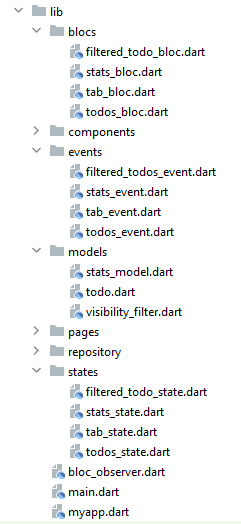
\includegraphics[width=0.4\textwidth]{Images/struttura_cartelle_bloc.png}
    \caption{Shows the final folders structure for the BLoC implementation of the Todos app}
    \label{fig:struttura_cartelle_bloc}
\end{figure}
Figure \ref{fig:widget_tree_structure_bloc} represents the widget's tree structure for the InheritedWidget final application. Notice the TodoProvider widget, situated below the HomePage, providing an instance of the TodoInheritedData to the subtree.

\begin{figure}[H]
    \centering
    \subfloat[Widgets tree structure \textit{todos }tab\label{fig:todos_tab_UI}]{
        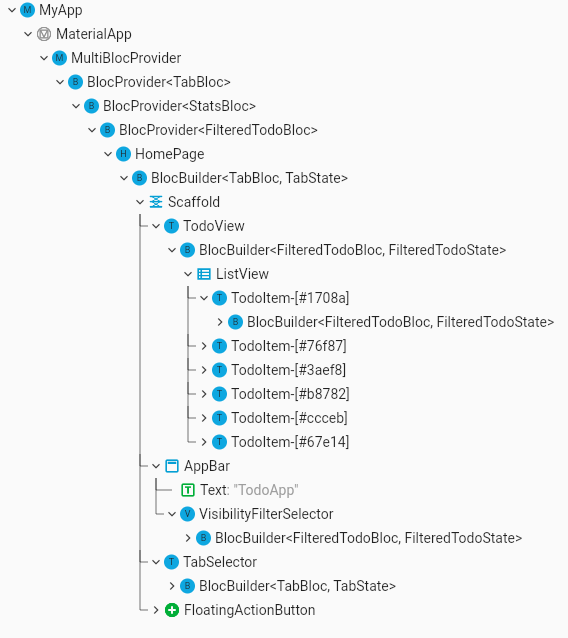
\includegraphics[scale=0.6]{Images/albero_bloc_todos.png}
    }
    \quad
    \subfloat[Widgets tree structure \textit{stats }tab\label{fig:todos_tab_tree}]{
        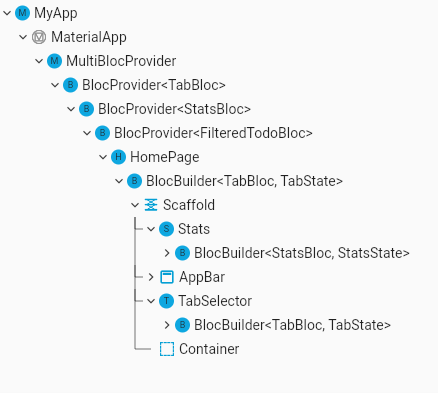
\includegraphics[scale=0.6]{Images/albero_bloc_stats.png}
    }
    \caption{Shows the widgets tree structure for BLoC Todos app}
    \label{fig:widget_tree_structure_bloc}
\end{figure}

